
%(BEGIN_QUESTION)
% Copyright 2006, Tony R. Kuphaldt, released under the Creative Commons Attribution License (v 1.0)
% This means you may do almost anything with this work of mine, so long as you give me proper credit

A {\it heat exchanger} is a metal device built to facilitate heat transfer between two fluids:

$$\includegraphics[width=15.5cm]{i00334x01.eps}$$

A {\it heating} fluid enters one side of the heat exchanger and gives up some of its thermal energy to the {\it heated} fluid on the other side of a thin, metal barrier.  The heated fluid, meanwhile, absorbs the heat released by the heating fluid across the barrier, increasing its temperature before exiting.

There are many different types of heat exchangers, but they all function on the same basic principles: thermal convection (heat transfer between each fluid and the barrier), and thermal conduction (heat transfer through the barrier itself). 

Suppose that a heat exchanger is being used to pre-heat fuel oil with steam prior to combustion in a boiler (this is common practice in boilers operating with heavy liquid petroleum fuel such as ``bunker-C''):

$$\includegraphics[width=15.5cm]{i00334x02.eps}$$

What will happen to the steam and oil outlet temperatures if the oil {\it flow} is decreased?  I'm looking for qualitative answers here (increase, decrease, or stay the same).


\underbar{file i00334}
%(END_QUESTION)





%(BEGIN_ANSWER)

If the oil flow rate decreases, its outlet temperature will increase because each oil molecule spends more time inside the heat exchanger, and thus has more time to absorb heat energy from the steam.  

The steam outlet temperature will increase as well, because the decreased flow of oil is not removing as much heat from the steam as it passes through.  One way to envision this is to think of the oil as cooling the steam, rather than the steam heating the oil.  With less oil entering the exchanger to cool the steam, the outgoing steam will be at a higher temperature than before.

%(END_ANSWER)





%(BEGIN_NOTES)


%INDEX% Physics, heat and temperature: heat exchangers

%(END_NOTES)


